\documentclass[12pt]{article}
\usepackage[margin=2cm, bindingoffset=0cm]{geometry}
%\usepackage[german]{babel} 
\usepackage[ngerman]{babel} %sudo apt-get install texlive-lang-german
\usepackage{hyperref} % web links etc.
\usepackage[parfill]{parskip}
\usepackage[utf8]{inputenc}
\usepackage[dvipsnames]{xcolor}
\usepackage{tcolorbox}
\usepackage{helvet} 
\usepackage{framed}
\usepackage{anyfontsize}
\usepackage{csquotes}
\usepackage{mathrsfs}
\usepackage{physics}
\setcounter{MaxMatrixCols}{16}
\usepackage{amssymb}
\usepackage{MnSymbol}
\MakeOuterQuote{"}
\definecolor{quotecolor}{rgb}{0.8,0.9,1}
\renewcommand{\familydefault}{\sfdefault} 
\setlength\parindent{0pt}
\tcbset{boxrule=0pt,colback=quotecolor,arc=5pt,auto outer arc,left=5pt,right=5pt,boxsep=5pt}
%  width=0.9\textwidth,

\setcounter{secnumdepth}{-1}
\begin{document}
\title{\fontsize{25}{25}\selectfont \textbf{Über psychische und physikalische Zeit}}
\author{Harald Rieder}
\date{\today}
\maketitle

%\begin{abstract}

%\end{abstract}

\tableofcontents

\section{Motivation}

Der Erfolg der relativistischen Physik lehrt uns, dass die Zeit irgendwie gleichrangig neben dem Ort zu stehen hat. Wechselt ein Beobachter seine Perspektive auf bestimmte Art, sehen  Koordinaten, die zuvor wie reine Ortskoordinaten ausgesehen haben, plötzlich ein wenig wie Zeitkoordinaten aus, und umgekehrt. Ein solcher Perspektiv-Wechsel heißt \emph{Lorentz-Transformation}. 

Der Alltag lehrt uns, dass die Zeit kontinuierlich vergeht, und zwar in eine bestimmte Richtung. Denn das Alltagsgeschehen scheint sich meistens nicht umkehren zu lassen. Eine zerschellte Tasse setzt sich nicht mit der Zeit wieder zu einer heilen Tasse zusammen und kehrt unter Abkühlung auf den Tisch zurück. Solches Alltagsgeschehen wird durch den 2. Hauptsatz der Thermodynamik erfolgreich modelliert.

Der Erfolg der Physik insgesamt lehrt uns, dass Ortsraum keine eingebaute Richtung hat. Es gibt keinen Satz der behauptet, dass wenn man in eine bestimmte Richtung geht, die Tassen immer kaputter werden müssen.

Somit haben wir 3 erfolgreich anwendbare Konzepte, die im Widerspruch zu stehen scheinen. Raum und Zeit sind wie Bruder und Schwester. Die Zeit hat aber eine eingebaute Richtung. Der Raum nicht. Und nun?

Darum schauen wir uns an, wozu uns ein paar unkonventionelle Annahmen führen können:

\begin{itemize}
\item In der Physik vergeht keine Zeit. Die Natur der physikalischen Zeit ist wie die Natur des physikalischen Ortsraums.
\item In der Psyche vergeht Zeit. Sie ist integraler Bestandteil des Bewusstwerdens, des Geistes. 
\item Es muss einen Mechanismus geben, der die psychische Zeit mit einem Bestandteil der physikalischen Welt so koppelt, dass es wenigstens für die menschliche Psyche den Anschein hat, die physikalische Zeit würde objektiv vergehen.
\end{itemize}

\section{Eine Quantenuhr}

In der Quantenmechanik spielt sich das Geschehen in einem vieldimensionalen Konfigurationsraum ab, dem Hilbert-Raum. Ein Ort existiert in diesem Raum zunächst nicht. Erst durch Festlegung auf eine Basis lassen sich komplexwertige Funktionen erstellen. Diese Funktionen stehen für unendlich viele Amplituden, die durch einen kontinuierlichen reellwertigen Index $x$ durchnummeriert werden.

Durch Beobachtung von außen, sowie durch Symmetrien, die wir aus der Erfahrung her einem dreidimensionalen Ortsraum zuschreiben, gelingt uns der Anschluss. Es sind unendlich viele Basen wählbar, doch nur bestimmte Wahlen führen zu einer Indexierung, bei der wir den Index als Ortskoordinate interpretieren können. Die Amplitude eines abstrakten Zustandsvektors $\ket{\psi}$ an einem bestimmten Ort liefert uns das Skalarprodukt mit dem abstrakten Vektor einer "Ortsbasis"
\begin{equation} 
\psi(x) \equiv \bra{x}\ket{\psi} 
\end{equation}
Wenn wir die physikalische Zeit ähnlich wie den Ort behandeln wollen, dann muss die Zeitkoordinate $t$ ebenso ein reellwertiger kontinuierlicher Index sein. Das heißt
\begin{equation} 
\label{eq:psi_xt}
\psi(x,t) \equiv \bra{x,t}\ket{\psi} 
\end{equation}
Die Indizes $x$ und $t$ nummerieren nun zusammen eine Produktbasis aus Orts- und Zeiteigenvektoren. Wir könnten aufgrund der Gleichmächtigkeit von $\mathbb{R}$ mit $\mathbb{R}^2$ diesen Index durch einen gemeinsamen reellwertigen Index $i = i(x,t)$ ersetzen und kämen damit wieder auf die Form
\begin{equation}
\psi(i) \equiv \bra{i}\ket{\psi} 
\end{equation}
wobei $\ket{\psi}$ wie in (\ref{eq:psi_xt}) der abstrakte Zustandsvektor im Produktraum ist.

Wir nehmen an, dass der Beobachter aus seinem Hilbert-Raum $\mathscr{H}_X$ heraus nicht in der Lage dazu ist, Zeit "direkt" in Erfahrung zu bringen. Diese Annahme drückt sich in der Quantenmechanik so aus, dass in Matrixelementen $H(X,x)$ von Wechselwirkungs-Hamiltonians die Zeit nicht auftritt. Ein Beobachter muss eine Zeigerstellung, einen Ort, ablesen, um von dort auf die Zeit im Uhrenzustand zu schließen. 

\begin{figure}[!h]\begin{center}
  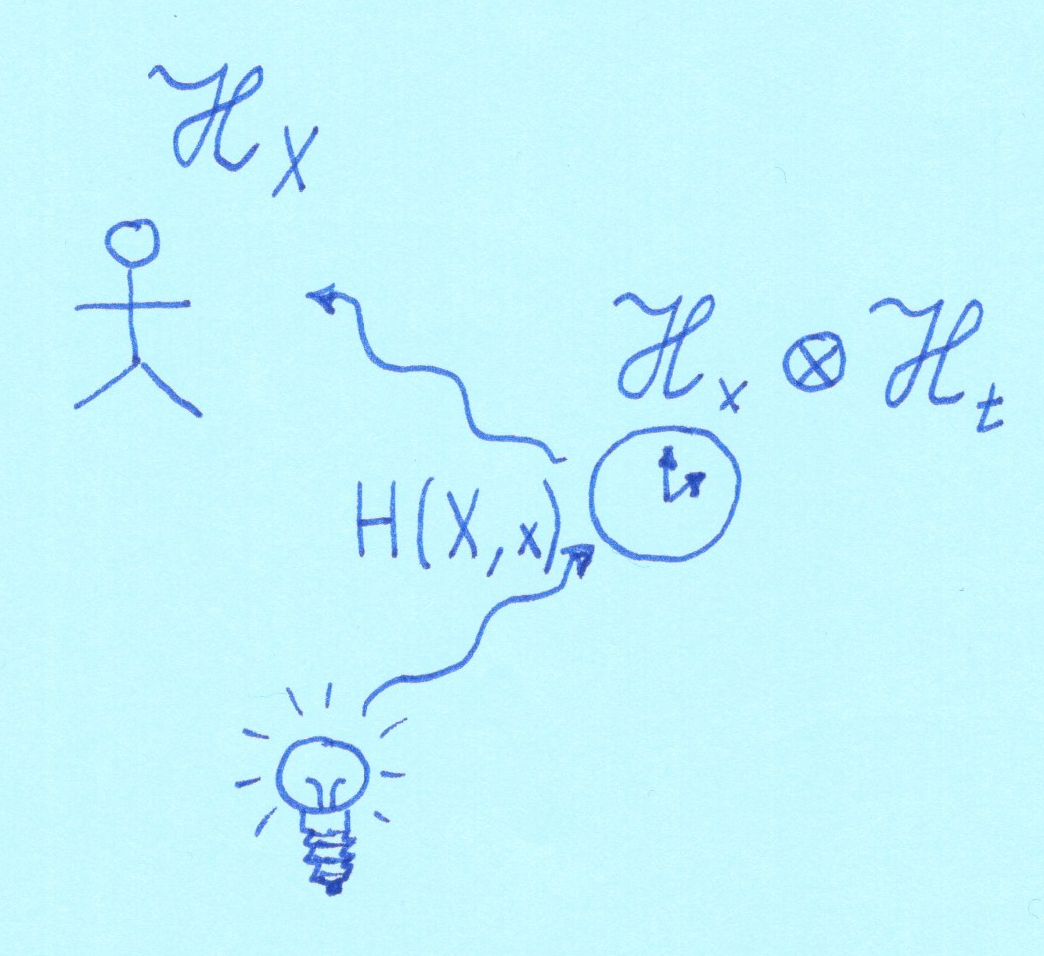
\includegraphics[width=6cm]{Quantenuhr.png}
  \caption{Indirektes Ablesen der Uhrzeit}
  \label{fig:sr_game}
\end{center}\end{figure}

Ein guter Uhrenzustand kann also ein Zustandsvektor im Produktraum $\mathscr{H}_x \otimes \mathscr{H}_t$ sein, der Orts- und Zeitunterräume maximal verschränkt. Wenn $\delta(x-\xi)$ die Amplituden von Ortseigenvektoren im Ortsunterraum in der Ortsdarstellung sind, und $\delta(t-\tau)$ die Amplituden von Zeiteigenvektoren im Zeitunterraum in der Zeitdarstellung, dann sind\footnote{Fortan lassen wir die Integralgrenzen weg, wenn sie im Unendlichen liegen.}
\begin{equation} 
\label{eq:psi_clock}
\psi(x,t) \sim \int_{-\infty}^{\infty} d\chi \delta(x-\chi) \delta(t-\chi) = \delta(x-t)
\end{equation}
die Amplituden eines maximal verschränkten Zustands, der aus der Beobachtung von $\xi$ sicher auf die Zeit $\tau$ schließen lässt. Durch die Beobachtung (oder Messung) "kollabiert die Überlagerung"
\begin{equation} 
\label{eq:collapse}
\int d\chi \delta(x-\chi) \delta(t-\chi) \quad \rightarrow \quad \delta(x-\chi)\delta(t-\chi)
\end{equation}
Dadurch ist die Uhr zunächst kaputtgegangen. Denn durch verträgliche Messungen, also wiederholte Ortsmessungen, werden wir immer wieder nur diesen Zustand und damit die Zeit $\chi$ antreffen. Es fehlt also ein Mechanismus, der die Uhr wieder scharfschaltet, sie in ihren verschränkten Zustand zurückbringt.

Im Artikel \emph{\href{https://docs.google.com/document/d/1OrmVETmnBSe5c0CpTbKH8Vq5pWFuB8QUez-KqHTaarQ/edit?usp=sharing}{Ideas about a Quantum Theory without Process Type 2}} wird so ein Mechanismus vorgestellt. Dort wird postuliert, dass jeder bewusste Beobachter einerseits eine Teilung des Hilbertraums vornimmt, andererseits die Änderung der Verschränkungen, wie sie erst durch die jeweilige Teilung aus den jeweils vorliegenden Zustandsvektoren entstehen, erlebt, ja sie sogar willentlich herbeiführen kann, wodurch dann \emph{aus Sicht des jeweiligen Beobachters} die quantenmechanische Überlagerung kollabiert und am Ende ein reiner Produktzustand vorliegt. Mindestens 2 solcherart an den physikalischen Kanal angeschlossene Beobachter (\emph{conscious splits}) sind notwendig, um ein Geschehen am Laufen zu halten. Unsere Uhr soll von einem äußeren Beobachter wie gezeigt hin und wieder abgelesen werden. Wir benötigen also noch einen weiteren "internen" Beobachter, der den x,t-Produktraum auf andere Weise teilen muss als der externe Beobachter. Der interne Beobachter teilt den Produktraum dazu nicht in x- und t-Basen, sondern in eine Basis aus x,t-verschränkten Zuständen und eine Basis, die den ganzen Rest enthält.

Um zu sehen, wie es läuft, betrachten wir ein einfaches Beispiel...

\section{Eine Quantenuhr aus 4 Qubits}

Unsere einfache Quantenuhr soll nur 4 diskrete Zeigerstellungen haben: $\ket{x=0}, \ket{x=1}, \ket{x=2}, \ket{x=3}$. Sie soll auch nur 4 Zeitpunkte messen können: $\ket{t=0}, \ket{t=1}, \ket{t=2}, \ket{t=3}$. Wir lassen jetzt der Übersichtlichkeit halber x und t weg, x soll links stehen, t rechts. Das heißt zum Beispiel $\ket{00}$ soll für $\ket{x=0}\ket{t=0}$ stehen. Wir haben es mit einem Produktraum aus 4 Qubits, 2 Raum- und 2 Zeit-Qubits zu tun. Für eine Orthogonalbasis der sind 16 Basisvektoren notwendig.

Der Unterraum aus maximal x,t-verschränkten Zuständen kann zum Beispiel durch diese 4 Basisvektoren aufgespannt werden
\begin{equation}
\begin{matrix}
??? evtl. nicht so
\ket{v_1} = {1}/{2} \, \left(\, \ket{00} + \ket{11} + \ket{22} \,\right) \\
\ket{v_2} = {1}/{2} \, \left(\, \ket{00} + \ket{11} - \ket{22} \,\right) \\
\ket{v_3} = {1}/{2} \, \left(\, \ket{00} - \ket{11} + \ket{22} \,\right) \\
\ket{v_4} = {1}/{2} \, \left(\, \ket{00} - \ket{11} + \ket{22} \,\right) ???
\end{matrix}
\end{equation}

\begin{equation}
\frac{1}{\sqrt{2}} \left(\, \ket{00} + \ket{11} \,\right)
\quad\quad\hat{=}\quad\quad
\frac{1}{\sqrt{2}}
\begin{pmatrix}
1 \\ 0 \\ 0 \\ 0 \\ 0 \\ 1 \\ 0 \\ 0 \\ 0 \\ 0 \\ 0 \\ 0 \\ 0 \\ 0 \\ 0 \\ 0
\end{pmatrix}
\quad
\begin{matrix}
00 \\ 01 \\ 02 \\ 03 \\ 10 \\ 11 \\ 12 \\ 13 \\ 20 \\ 21 \\ 22 \\ 23 \\ 30 \\ 31 \\ 32 \\ 33 
\end{matrix}
\end{equation}

\begin{equation}
U\ =\ 
\begin{pmatrix}
\pmb{\frac{1}{2}} &&&&& \pmb{0} &&&&& \pmb{\frac{1}{2}} &&&&& \pmb{\frac{\sqrt{2}}{2}} \\
  & 1 &   &   &   &   &   &   &   &   &   &   &   &   &   &   \\
  &   & 1 &   &   &   &   &   &   &   &   &   &   &   &   &   \\
  &   &   & 1 &   &   &   &   &   &   &   &   &   &   &   &   \\
  &   &   &   & 1 &   &   &   &   &   &   &   &   &   &   &   \\
\pmb{\frac{\sqrt{2}}{2}} &&&&& \pmb{\frac{1}{2}} &&&&& \pmb{0} &&&&& \pmb{-\frac{1}{2}} \\
  &   &   &   &   &   & 1 &   &   &   &   &   &   &   &   &   \\
  &   &   &   &   &   &   & 1 &   &   &   &   &   &   &   &   \\
  &   &   &   &   &   &   &   & 1 &   &   &   &   &   &   &   \\
  &   &   &   &   &   &   &   &   & 1 &   &   &   &   &   &   \\
\pmb{-\frac{1}{2}} &&&&& \pmb{\frac{\sqrt{2}}{2}} &&&&& \pmb{\frac{1}{2}} &&&&& \pmb{0} \\
  &   &   &   &   &   &   &   &   &   &   & 1 &   &   &   &   \\
  &   &   &   &   &   &   &   &   &   &   &   & 1 &   &   &   \\
  &   &   &   &   &   &   &   &   &   &   &   &   & 1 &   &   \\
  &   &   &   &   &   &   &   &   &   &   &   &   &   & 1 &   \\
\pmb{0} &&&&& \pmb{-\frac{1}{2}} &&&&& \pmb{\frac{\sqrt{2}}{2}} &&&&& \pmb{-\frac{1}{2}} 
\end{pmatrix}
\quad
\begin{matrix}
00 \\ 01 \\ 02 \\ 03 \\ 10 \\ 11 \\ 12 \\ 13 \\ 20 \\ 21 \\ 22 \\ 23 \\ 30 \\ 31 \\ 32 \\ 33 
\end{matrix}
\end{equation}



\begin{equation}
\begin{matrix}
\ket{00}_{ext} \ \xrightarrow{U} \ \frac{1}{2}\ket{00}_{int} + \frac{\sqrt{2}}{2}\ket{11}_{int} + \frac{1}{2}\ket{22}_{int} 
& \xrightarrow{p = 0.25} & \ket{00}_{int} \\ \\
& \xrightarrow{p = 0.5} & \ket{11}_{int} \\ \\
& \xrightarrow{p = 0.25} & \ket{22}_{int}
\end{matrix}
\end{equation}



\begin{equation}
U^{-1}\ =\ 
\begin{pmatrix}
\pmb{\frac{1}{2}} &&&&& \pmb{\frac{\sqrt{2}}{2}} &&&&& \pmb{-\frac{1}{2}} &&&&& \pmb{0} \\
  & 1 &   &   &   &   &   &   &   &   &   &   &   &   &   &   \\
  &   & 1 &   &   &   &   &   &   &   &   &   &   &   &   &   \\
  &   &   & 1 &   &   &   &   &   &   &   &   &   &   &   &   \\
  &   &   &   & 1 &   &   &   &   &   &   &   &   &   &   &   \\
\pmb{0} &&&&& \pmb{\frac{1}{2}} &&&&& \pmb{\frac{\sqrt{2}}{2}} &&&&& \pmb{-\frac{1}{2}} \\
  &   &   &   &   &   & 1 &   &   &   &   &   &   &   &   &   \\
  &   &   &   &   &   &   & 1 &   &   &   &   &   &   &   &   \\
  &   &   &   &   &   &   &   & 1 &   &   &   &   &   &   &   \\
  &   &   &   &   &   &   &   &   & 1 &   &   &   &   &   &   \\
\pmb{\frac{1}{2}} &&&&& \pmb{0} &&&&& \pmb{\frac{1}{2}} &&&&& \pmb{\frac{\sqrt{2}}{2}} \\
  &   &   &   &   &   &   &   &   &   &   & 1 &   &   &   &   \\
  &   &   &   &   &   &   &   &   &   &   &   & 1 &   &   &   \\
  &   &   &   &   &   &   &   &   &   &   &   &   & 1 &   &   \\
  &   &   &   &   &   &   &   &   &   &   &   &   &   & 1 &   \\
\pmb{\frac{\sqrt{2}}{2}} &&&&& \pmb{-\frac{1}{2}} &&&&& \pmb{0} &&&&& \pmb{-\frac{1}{2}} 
\end{pmatrix}
\quad
\begin{matrix}
00 \\ 01 \\ 02 \\ 03 \\ 10 \\ 11 \\ 12 \\ 13 \\ 20 \\ 21 \\ 22 \\ 23 \\ 30 \\ 31 \\ 32 \\ 33 
\end{matrix}
\end{equation}

\begin{equation}
\begin{matrix}
\ket{00}_{int} \ \xrightarrow{U^{-1}} \ \frac{1}{2}\ket{00}_{ext} + \frac{1}{2}\ket{22}_{ext} + \frac{\sqrt{2}}{2}\ket{33}_{ext} 
& \xrightarrow{p = 0.25} & \ket{00}_{ext} \\ \\
& \xrightarrow{p = 0.25} & \ket{22}_{ext} \\ \\
& \xrightarrow{p = 0.5} & \ket{33}_{ext}
\end{matrix}
\end{equation}
\begin{equation}
<t>_{\ket{00}_{int}} \ = \  0.25 \cdot 0 + 0.25 \cdot 2 + 0.5 \cdot 3 = 2
\end{equation}

\begin{equation}
\begin{matrix}
\ket{11}_{int} \ \xrightarrow{U^{-1}} \ \frac{\sqrt{2}}{2}\ket{00}_{ext} + \frac{1}{2}\ket{11}_{ext} - \frac{1}{2}\ket{33}_{ext} 
& \xrightarrow{p = 0.5} & \ket{00}_{ext} \\ \\
& \xrightarrow{p = 0.25} & \ket{11}_{ext} \\ \\
& \xrightarrow{p = 0.25} & \ket{33}_{ext}
\end{matrix}
\end{equation}
\begin{equation}
<t>_{\ket{11}_{int}} \ = \  0.5 \cdot 0 + 0.25 \cdot 1 + 0.25 \cdot 3 = 0.\overline{3}
\end{equation}

\begin{equation}
\begin{matrix}
\ket{22}_{int} \ \xrightarrow{U^{-1}} \ -\frac{1}{2}\ket{00}_{ext} + \frac{\sqrt{2}}{2}\ket{11}_{ext} + \frac{1}{2}\ket{22}_{ext} 
& \xrightarrow{p = 0.25} & \ket{00}_{ext} \\ \\
& \xrightarrow{p = 0.5} & \ket{11}_{ext} \\ \\
& \xrightarrow{p = 0.25} & \ket{22}_{ext}
\end{matrix}
\end{equation}
\begin{equation}
<t>_{\ket{22}_{int}} \ = \  0.25 \cdot 0 + 0.5 \cdot 1 + 0.25 \cdot 2 = 1.50
\end{equation}




\section{Das Anwachsen der Entropie in der psychischen Zeit}


\section{Eine relativbewegte Quantenuhr}

Wir fragen nun danach, wie eine bewegte Uhr gesehen wird. Wenn der externe Beobachter die Zeigerstellung $\chi$ erkennt, dann schließt er daraus, dass in der bewegten Uhr die Zeit $\chi$ vergangen ist. Daran ändert eine Relativbewegung der Uhr nichts. Das heißt, eine Relativbewegung soll nichts daran ändern, welche Ortseigenvektoren mit welchen Zeiteigenvektoren verschränkt sind. Im diskreten Fall kann sich also an der Verschränkung gar nichts ändern. Im Raumzeitkontinuum gibt es dagegen mehr Freiheit. Wir greifen zurück auf den kontinuierlichen Uhrenzustand (\ref{eq:psi_clock}). 

Eine Koordinatentransformation der internen Uhrkoordinaten $x,t$ auf die Koordinaten $x',t'$ aus Sicht des externen Beobachters soll also bewirken
\begin{equation} 
\psi(x,t) \sim \delta(x-t)\ \longmapsto \ \psi(x',t') \sim \delta(x'-t')
\end{equation} 
Bemerkenswerterweise ist ein Lorentz-Boost in x-Richtung solch eine verschränkungserhaltende Transformation, denn
\begin{equation} 
\delta(x'-t') =\, \delta(\gamma (x + \beta t) - \gamma (t + \beta x)) 
= \frac{\delta(x-t)}{\gamma (1-\beta)} \sim \delta(x-t)
\end{equation}
wenn wir t in Metern messen, was wir schon von Anfang an getan haben. Allerdings trifft das für Uhrenzeigerkoordinaten in y- oder z-Richtung nicht zu, da bei einem Boost in x-Richtung $y'=y$ und $z'=z$ gilt.
\end{document}
